\chapter{機械学習を用いた Coincidence Window の作成手法}
本章では本研究の主題である機械学習を用いた CW の作成手法について述べる。

\section{機械学習}\label{回帰分析}
機械学習は近年大きな注目を集めている技術であり、本研究の目的である CW の作成作業の効率化に対する解決案として期待できる。
ここで機械学習とは、データからコンピュータが自動で特徴量やルールを学習し、学習した結果に基づいて新たなデータに対し分類や予測を行う分析手法の一つである。
代表的な分析手法として「クラス分類」と「回帰分析」がよく知られている。
回帰の主な目的は、連続値などの値を学習データの傾向をもとに予測することである。過去の気温から明日の気温を予測することや企業における売り上げの予測などが回帰に当てはまる。回帰分析には、線形回帰、多項式回帰などが存在し、図\ref{fig:regre}に線形回帰の概要図を示す。
一方で分類は、分析したいデータが属するカテゴリーやクラス、種類が何なのかを判定する手法である。特に、予測するクラス数が 2 クラスの場合には 2 値分類と、2クラスより多い分類予測については多クラス分類と呼ばれる。図\ref{fig:class}にクラス分類の概要図を示す。
\begin{figure}[tb]
  \centering
    \begin{minipage}[b]{0.4\linewidth}
        \centering
        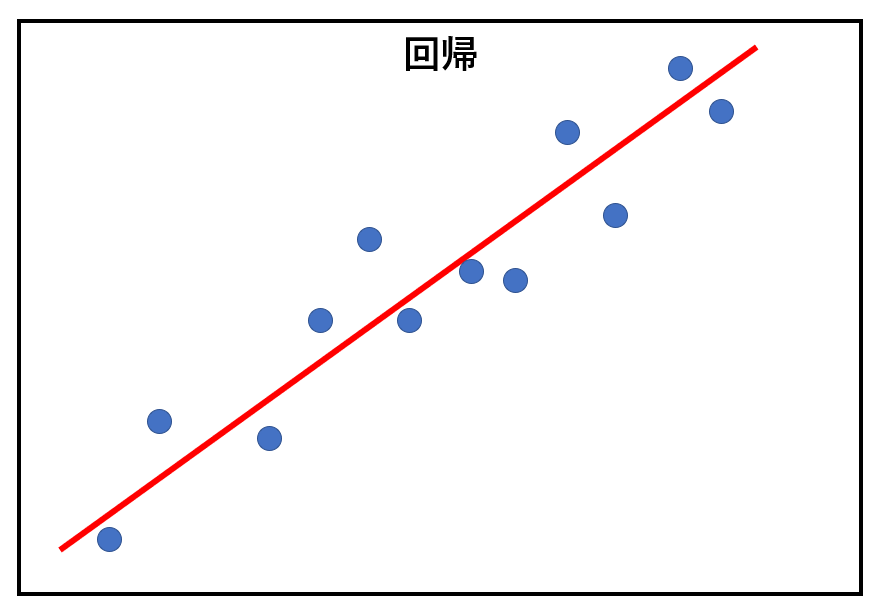
\includegraphics[clip, width=7cm]{fig/4/regression.png}
        \vspace{10pt}
        \subcaption{}
        \label{fig:regre}
    \end{minipage}
    \hfill
    \begin{minipage}[b]{0.4\linewidth}
        \centering
        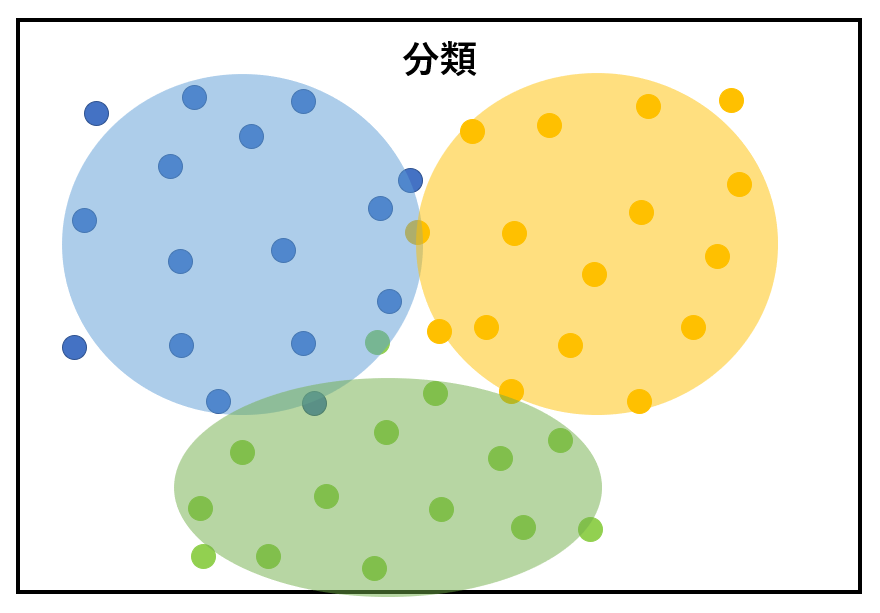
\includegraphics[clip, width=7cm]{fig/4/classification.png}
        \vspace{10pt}
        \subcaption{}
        \label{fig:class}
    \end{minipage}
  \caption{機械学習の代表的な分析手法。(a):回帰分析、(b):クラス分類の概要図}
  \label{fig:fit_def}
\end{figure}

機械学習の学習手法は、教師あり学習、教師なし学習、強化学習の 3 つに大きく分けられる。
教師あり学習は正解の値を与えた状態で傾向を学習させる方法である。
教師あり学習は、「学習」と「予測」といった 2 つのプロセスによって成り立っており、、正解のデータを用いてルールやパターンの学習を行った後、新しいデータに対して、これまでに学習したデータを用いて予測を行う。
一方で教師なし学習は、正解の値を教えずに学習させる方法である。大量のデータを学習させることでデータの特徴やパターンなどを覚えるが、それが正解か否かを判断することを学ぶのが教師なし学習の特徴である。
また強化学習では、出力される結果に点数をつけて、最も多くの点数を得るための行動を学習させる。教師なし学習と同じように正解の値を学習させないが、教師なし学習との違いは、機械が報酬を得るために最適な行動を自ら考え実行する点である。

\subsection{ニューラルネットワーク}
機械学習には多くの種類があるが、その内の一つがニューラルネットワークを使った手法である。ニューラルネットワークとは、人間の脳内にある神経細胞(ニューロン)とそのつながり、つまり神経回路網を人工ニューロン(パーセプトロン)という数式的なモデルで表現したものである。個々のパーセプトロンは単純な仕組みであるが、多数組み合わせる事で複雑な関数近似を行う事ができるのが、ニューラルネットワークの大きな特徴である。

図\ref{fig:perce}に示すように、パーセプトロンは入力と出力の2層で構成され、 n 個の信号$x_i$に対し重み$w_i$を作用させバイアス b とともに入力し、 1 個の信号$y$を出力する関数 $f(x_i, w_i)$ を持ったモデルである。式\eqref{equ:acctivation}で表すことができる。この $f(x_i, w_i)$ の事を「活性化関数」と呼び、活性化関数には、sigmoid 関数、tanh 関数、 ReLU 関数(Rectified linear Unit)」、 softmax 関数などが良く使われている。 
\begin{equation}
    y = f(\Vec{w}・\Vec{x} + b)
    %y = f(\sum^{n-1}_{i=1}(w_i・x_i) + b)
    %f \begin{pmatrix}  \\ 2 & 3 \end{pmatrix}
    \label{equ:acctivation}
\end{equation}
\begin{figure}[tb]
  \centering
  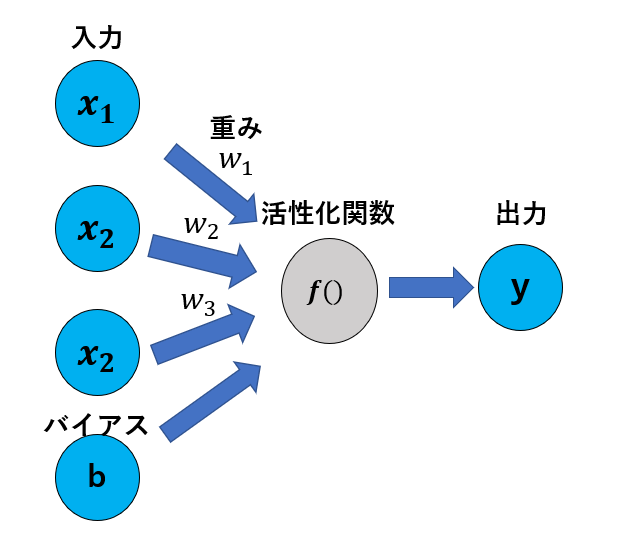
\includegraphics[clip, width=13cm]{fig/4/parceptron.png}
  \caption{パーセプトロン}
  \label{fig:perce}
\end{figure}
sigmoid 関数及びReLU 関数の概形を図\ref{fig:sigmoid},図\ref{fig:ReLU}に示す。sigmoid 関数はニューラルネットワークでよく用いられてきた関数であり、式\eqref{equ:sigmoid}のような関数で表される。ReLU 関数は式\eqref{equ:ReLU}のような関数で示される。
\begin{equation}
    y = \frac{1}{1+exp(-x)}
    %f \begin{pmatrix}  \\ 2 & 3 \end{pmatrix}
    \label{equ:sigmoid}
\end{equation}

\begin{equation}
    y = max(0,x)
    %f \begin{pmatrix}  \\ 2 & 3 \end{pmatrix}
    \label{equ:ReLU}
\end{equation}
\begin{figure}
    \centering
    \begin{minipage}[b]{0.4\linewidth}
        \centering
        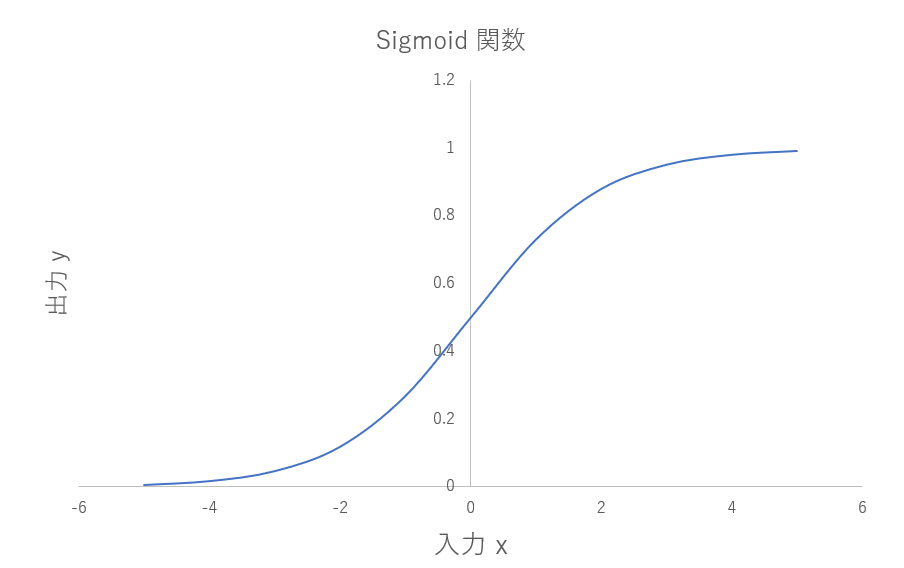
\includegraphics[clip, width=7cm]{fig/4/sigmoid.png}
        \vspace{10pt}
        \subcaption{}
        \label{fig:sigmoid}
    \end{minipage}
    \hfill
    \begin{minipage}[b]{0.4\linewidth}
        \centering
        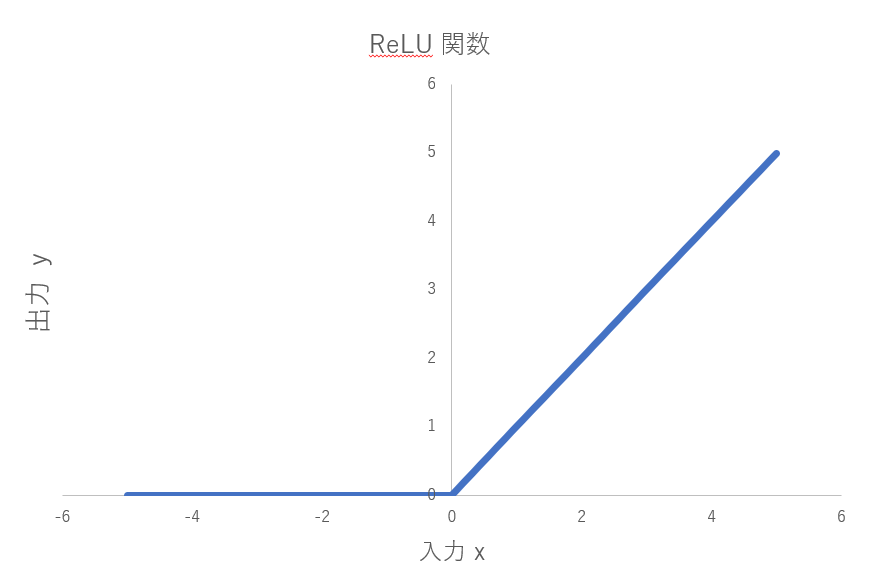
\includegraphics[clip, width=7cm]{fig/4/ReLU.png}
        \vspace{10pt}
        \subcaption{}
        \label{fig:ReLU}
    \end{minipage}
    \caption{機械学習で用いられる活性化関数の例。(a): sigmoid 関数、(b): ReLU 関数。}
    \label{fig:acctivation}
\end{figure}
単一のパーセプトロンでの分析は単純なものであれば問題ないが、複雑な事象を扱うことは難しい。そこで、このパーセプトロンを複数組み合わせることにより多層化することで、複雑な表現を可能とした多層パーセプトロン (MLP : Multilayer perceptron) が考案された。
単一のパーセプトロンは入力と出力のみであったのに対し、図\ref{fig:MLP}に示すように、MLP は隠れ層と呼ばれる層が複数追加されたネットワーク構造を持ち、各層間は全結合しているような構造になっている。この様な構造を持つニューラルネットワークの事を「全結合型ニューラルネットワーク」と呼ぶ。出力層においてよく使われる主な活性化関数としては、2種類の分類問題に対しては sigmoid 関数、多クラスの分類問題に対しては softmax 関数、回帰問題に対しては linear 関数などが用いられる。
\begin{figure}[tb]
  \centering
  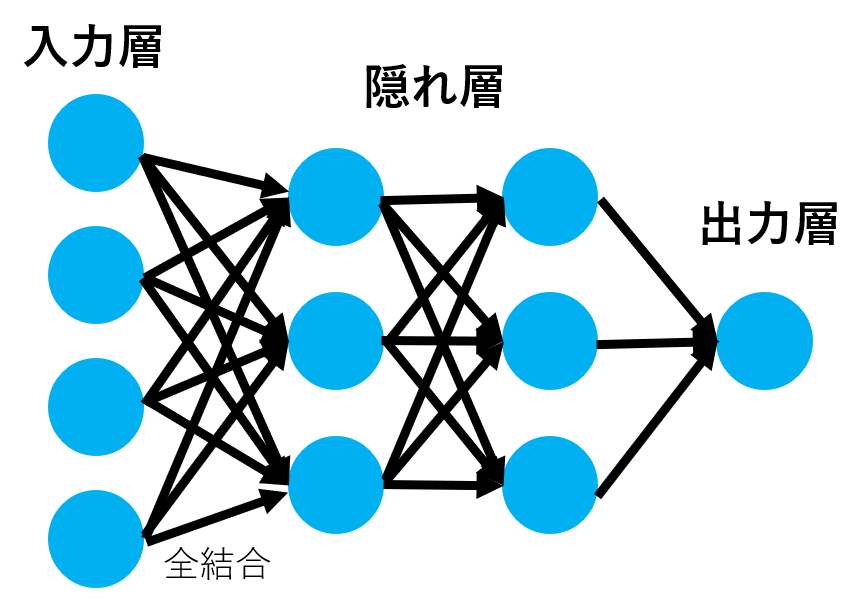
\includegraphics[clip, width=10cm]{fig/4/MLP_re.png}
  \caption{MLP の概形。パーセプトロンを複数組み合われており、ある層のパーセプトロンからの出力は全結合されて次の層の各パーセプトロンに入力される。}
  \label{fig:MLP}
\end{figure}

出力された予測値は損失関数を用いて評価が行われる。これは、入力値 $x_n$ に対してとある重み $w$ を設定して予測値 $y$ を導出し、その予測値 $y$ に対し目標値 $t$ との誤差 $L$ が最小になるようにそれぞれの重みやバイアスなどのパラメータの値を少しだけ増減させ調整を行う方法である。この調整を繰り返すことによって予測の精度を向上させていく。図\ref{fig:lossfunction}にパラメータの更新の流れを示す。
この調整の際に使用される誤差を計算する関数は「損失関数」と呼ばれ、特に式\eqref{equ:MSE}に示すような関数で表される平均二乗誤差(MSE : Mean Squared Error)が多く用いられる。他には、平均絶対誤差(MAE : Mean Absolute Error))や平均二乗誤差の平方根(RMSE : Root Mean Squared Error)などが用いられる。
\begin{equation}
    L = \frac{1}{n}\sum^{n}_{i=1}(y_i-t_i)^2
    %f \begin{pmatrix}  \\ 2 & 3 \end{pmatrix}
    \label{equ:MSE}
\end{equation}

\begin{figure}[tb]
  \centering
  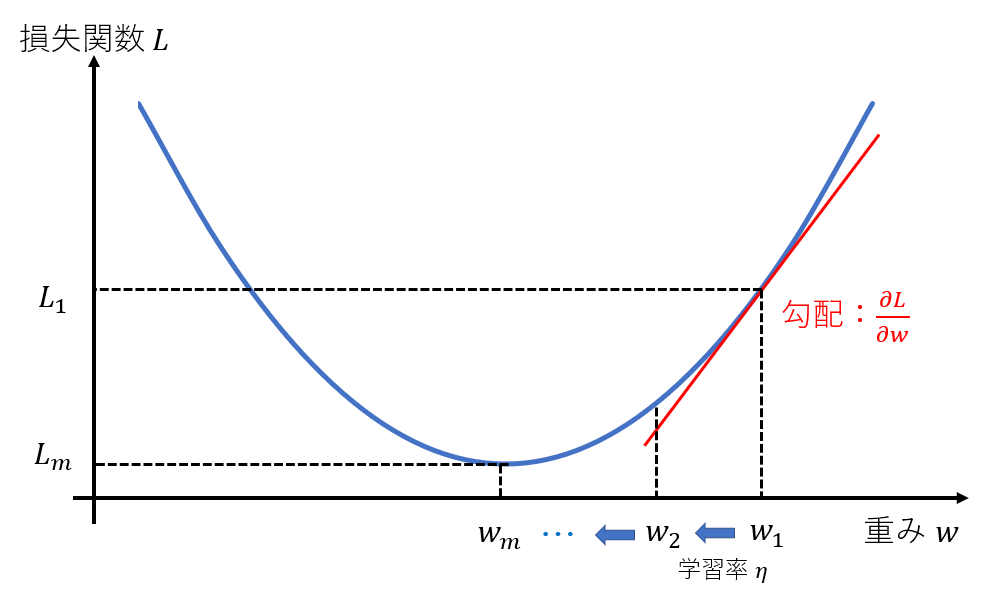
\includegraphics[clip, width=10cm]{fig/4/lossfunc_laerning.png}
  \caption{損失関数 $L$ の最小化の流れ。ある重み $w_i$ の時の勾配 $\frac{\partial L}{\partial w}$ を計算し、この勾配が小さくなるように重みを更新することを繰り返す。この際、更新量を調整するために学習率 $\eta$ を設定する。バイアス $b$ に対しても同様に最小化を行う。}
  \label{fig:lossfunction}
\end{figure}

\section{機械学習を用いた CW 作成手法}
本節では機械学習の学習方法及び CW を作成する手法について述べる。
従来の作成手法では、シミュレーションデータを用いて$p_T$閾値を決定し CW を作成する。その後、実際のデータを使用して磁場の影響や検出器のズレに最適化させるといった方法を行っていた。一方、本研究で開発する作成手法では実際のデータを学習に利用した機械学習を用いて$p_T$の値の予測を行い 、CW の作成と最適化を同時に行う。
本研究で作成する CW はシミュレーションで用いるトリガー用と実際の測定で用いるトリガー用の 2 種類であり、それぞれシミュレーションデータと実際のデータを使用し機械学習のトレーニングを行う。
教師データとしてはオフラインで再構成されたミューオンの横方向運動量を使用する。トレーニングデータの総数は 500 万イベントである。

初めに、入力に使用するシミュレーションデータおよび実際のデータを学習に適した形式に変更する。次にトリガーセクターの場所とRoI、飛跡の曲がり具合を表す($\Delta R$, $\Delta \phi$)に対応した$p_T$の値を出力する機械学習モデルをトレーニングする。本研究では、図\ref{fig:MLP_over}に示すような、ミューオンのヒット位置を示す RoI, トリガーセクターの情報とミューオンの飛跡の曲がり具合 $\Delta R$, $\Delta \phi$ の 4 変数を入力値として、横方向運動量$p_T$を出力とした MLP を用いる。分析手法として回帰分析を行うため、出力される$p_T$の値は連続値である。最後に、任意の$p_T$で区切った際のトリガー効率を求め、Turn-on curve にフィッティングを行い 15 段階の $p_T$ 閾値に対応した CW を作成する。

\begin{figure}[tb]
  \centering
  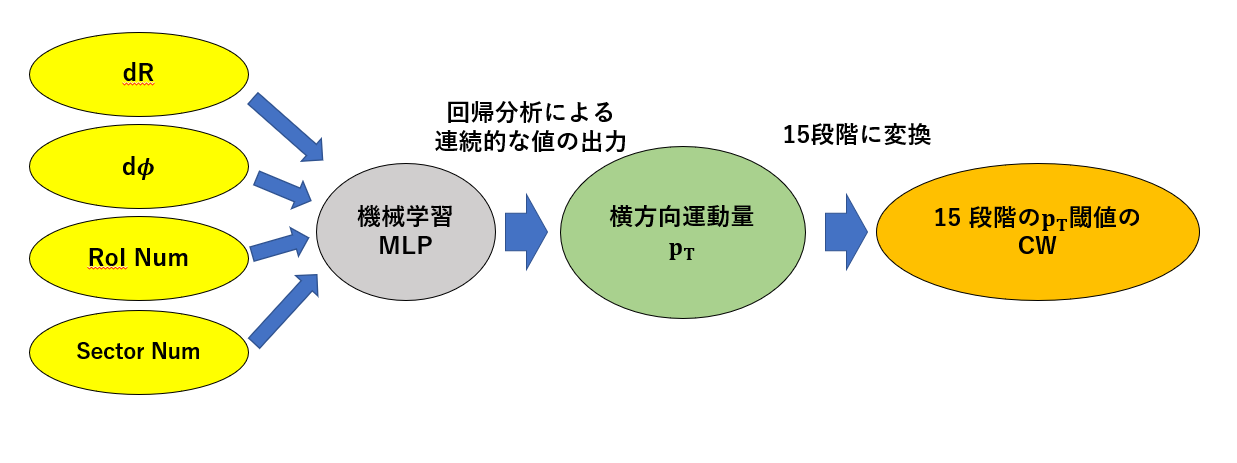
\includegraphics[clip, width=15cm]{fig/4/MLPoverview.png}
  \caption{機械学習を用いた CW 作成の流れ。$\Delta R$, $\Delta \phi$ RoI, トリガーセクターの情報の 4 変数を入力値、横方向運動量$p_T$を出力値とした機械学習を用いる。出力された$p_T$は連続値であり、これを15段階の$p_T$閾値に変換することで CW を作成する。}
  \label{fig:MLP_over}
\end{figure}

\subsection{入力データに対する事前処理}
本節では学習に用いる入力データに対する事前処理について述べる。

シミュレーション用の機械学習のトレーニングには、1 イベントにミューオンが 1 個存在するシミュレーションサンプル(シングルミューオンサンプル)を使用し、実際の測定用の機械学習のトレーニングには、2018年 Run-2 のデータを用いた。

\subsubsection{磁場構造を考慮した学習領域の分割}
\ref{magnetic_filed}節で述べたように、トロイド磁石が 8 回転対象に設置されていることにより TGC$\_$BW における磁場構造は図\ref{fig:Mag}に示すように一様ではない。そのため、本研究では TGC$\_$BW 全体を一括で学習させるのではなく、図\ref{fig:Mag}で示すように、入力データとして使用する領域を分割して学習を行う。
本研究では、磁場構造に考慮するためにTGC のエンドキャプ部を $\phi$ 方向に 48 分割、$\eta$ 方向に 9 分割、フォワード部を $\phi$ 方向に 24 分割、$\eta$ 方向に 4 分割にした。
\begin{figure}[tb]
  \centering
  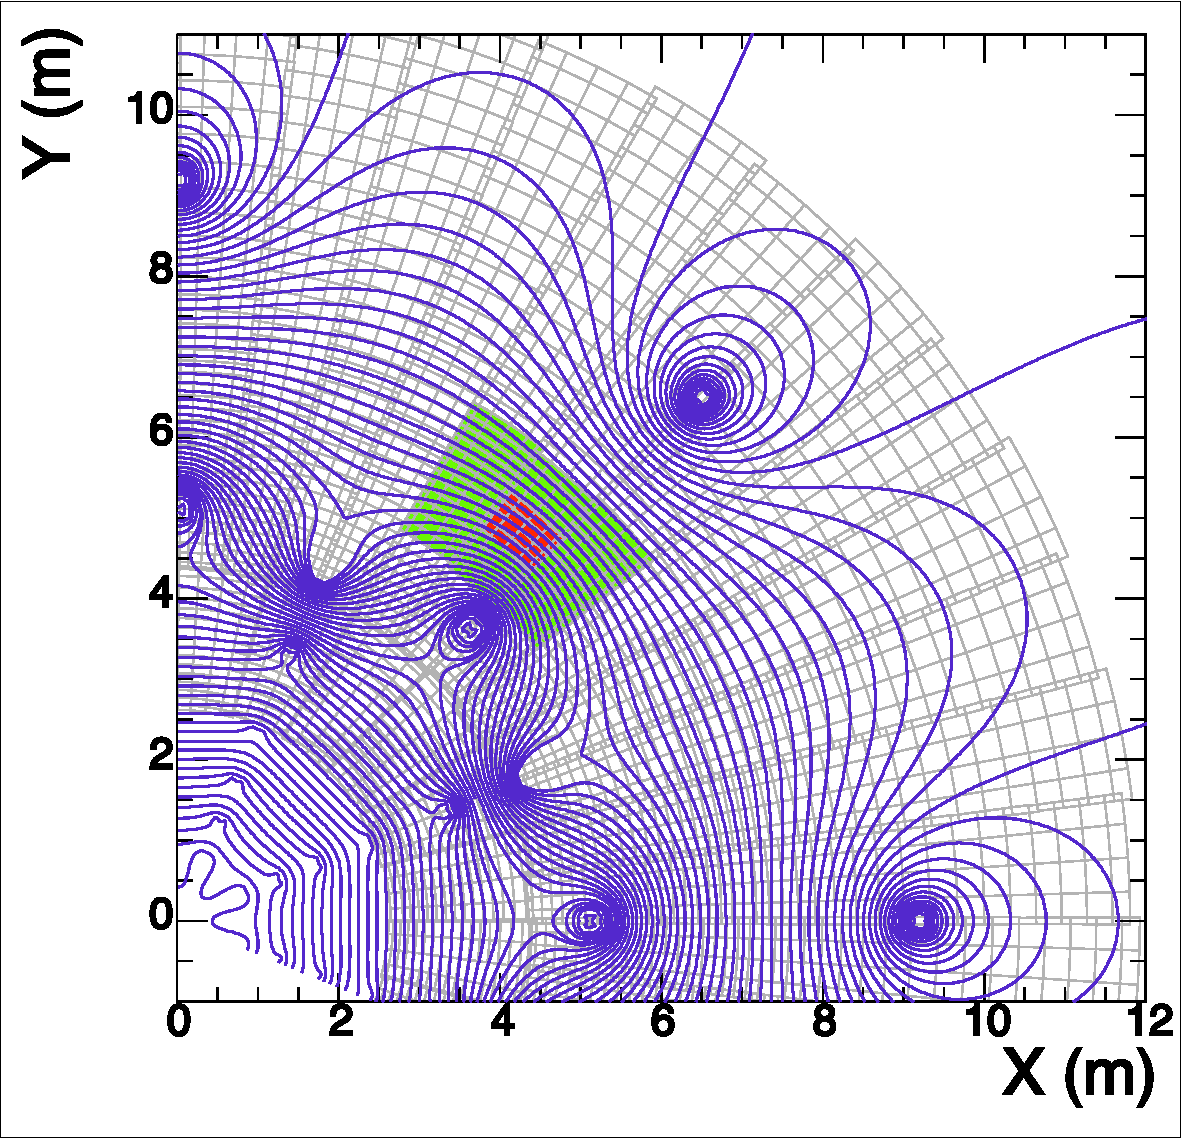
\includegraphics[clip, width=9cm]{fig/4/c1_withMag.pdf}
  \caption{磁場構造を考慮するための学習領域の分け方。「赤」の領域に対する学習を行う際には「赤」と「緑」の領域のデータのみを使用する。}
  \label{fig:Mag}
\end{figure}

\subsubsection{ミューオン情報の選別}
次に分割した入力データを用いて各 RoI に対するヒットマップを作成しミューオンの選別を行う。作成したヒットマップには孤立しているマス、穴の空いているマスが存在する。これは偶発的にミューオンヒットしたことや多重散乱の影響によるもので機械学習のトレーニングの際にノイズとなる。そのため、以下に説明するヒットマップクリーナーを用いてヒットマップの最適化を行う。
\begin{enumerate}
   \item エントリー数が 3 以下のビンは削除する。これは、偶発的にミューオンがヒットしたマスを削除することを目的とする。
   \item ミューオンがヒットしたマスが隣接する 8 個のマスのうち 2 つ以下であるとき、そのマスは削除する。孤立したミューオンのヒットを削除することを目的としている。
\end{enumerate}
入力データのヒットマップに対して、上記のヒットマップクリーナーの手順を 1 番から順番に要求し、ヒットマップを最適化を行う。図\ref{fig:hitmapcleaner}にヒットマップクリーナを作用させた場合の例を示す。

\begin{figure}[tb]
  \centering
  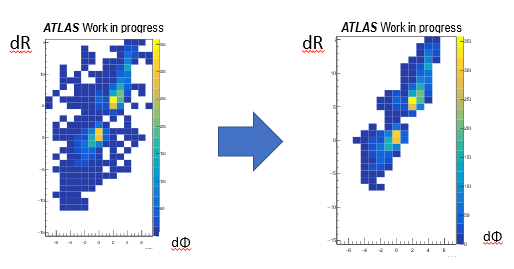
\includegraphics[clip, width=14cm]{fig/4/cleaner.png}
  \caption{ヒットマップクリーナーをかけた前後のミューオンヒットマップの例}
  \label{fig:hitmapcleaner}
\end{figure}


\subsection{機械学習モデルの設計方法とトレーニング}
本節では飛跡の曲がり具合と TGC$\_$BW のヒット情報からミューオンの横方向運動量 $p_T$ を出力させる機械学習モデルの設計について述べる。

\subsubsection{機械学習モデルの設計}

本研究において、機械学習モデルの構築には Google 社によって開発された機械学習に用いるためのオープンソースのフレームワークである TensorFlow \cite{article:TensorFlow}とニューラルネットワークライブラリである Keras \cite{article:keras}を用いた。

本研究で使用する機械学習モデルは、4 つの入力変数を持つ入力層、5 つの隠れ層、$p_T$ の値を出力する1 つの出力層となるような回帰分析を行う全結合型 MLP モデルを構築する。
図\ref{fig:MLP_overview}に機械学習モデルの概要図を示す。
MLP の各隠れ層は以下の表\ref{table:hibben}に示す要素から構成される。
\begin{enumerate}\label{table:hibben}
   \item Dence layer:前の層からのすべての出力の線形結合を入力としたパーセプトロンの層。1 つの層に存在するパーセプトロンの数をノード数と呼ぶ。
   \item Batch normalization layer:入力に対し正規化を行う層。
   \item Dropout unit:学習中にランダムに選ばれたノードの一定割合をゼロにする操作。過学習の抑制のために用いられ、ドロップアウトする割合はハイパーパラメータとして設定する。
   \item Activation unit:活性化関数を設定する層。本研究では Sigmoid 関数を選した。
   %\caption{隠れ層を構成する要素。}
\end{enumerate}
出力層には ReLU 関数を活性化関数として使用する。これは、目的とする $p_T$ の値が必ず正の値を取ることが確定しているためである。
誤差逆伝搬法には RMSprop optimizer を用いて勾配降下法を行っている。

\subsubsection{ハイパーパラメータ}
隠れ層の数、ノード数、ドロップアウト率、損失関数、学習率の 5 個のハイパーパラメータを表\ref{table:hyper}のように変化させることで評価を行い最適なモデルを選択した。評価にはPreferred Networks社が開発したハイパーパラメータの最適化を自動で行うフレームワークである Optuna \cite{article:optuna}を使用した。
\begin{enumerate}\label{table:hyper}
   \item 隠れ層の数:3層 \~ 7層
   \item ノード数:128, 256, 512, 1024
   \item ドロップアウト率:0.1, 0.2, 0.3, 0.4, 0.5
   \item 損失関数:MSE, MAS
   \item 学習率:0.01, 0.001, 0.0001
   %\caption{変化させるハイパーパラメータの一覧。}
\end{enumerate}
評価を行った結果、いくつかの組み合わせで同等の性能が得られることがわかった。これらのうち、学習可能なパラメータの数が最も少ないネットワークが選ばれた。パラメータとその値は、ドロップアウト率 0.2、損失関数 MSE、学習率 0.001, そして、5つの隠れ層と [512, 512, 512, 512, 512] のノード数を選択する。

\begin{figure}[tb]
  \centering
  %\rule{8cm}{6cm}
  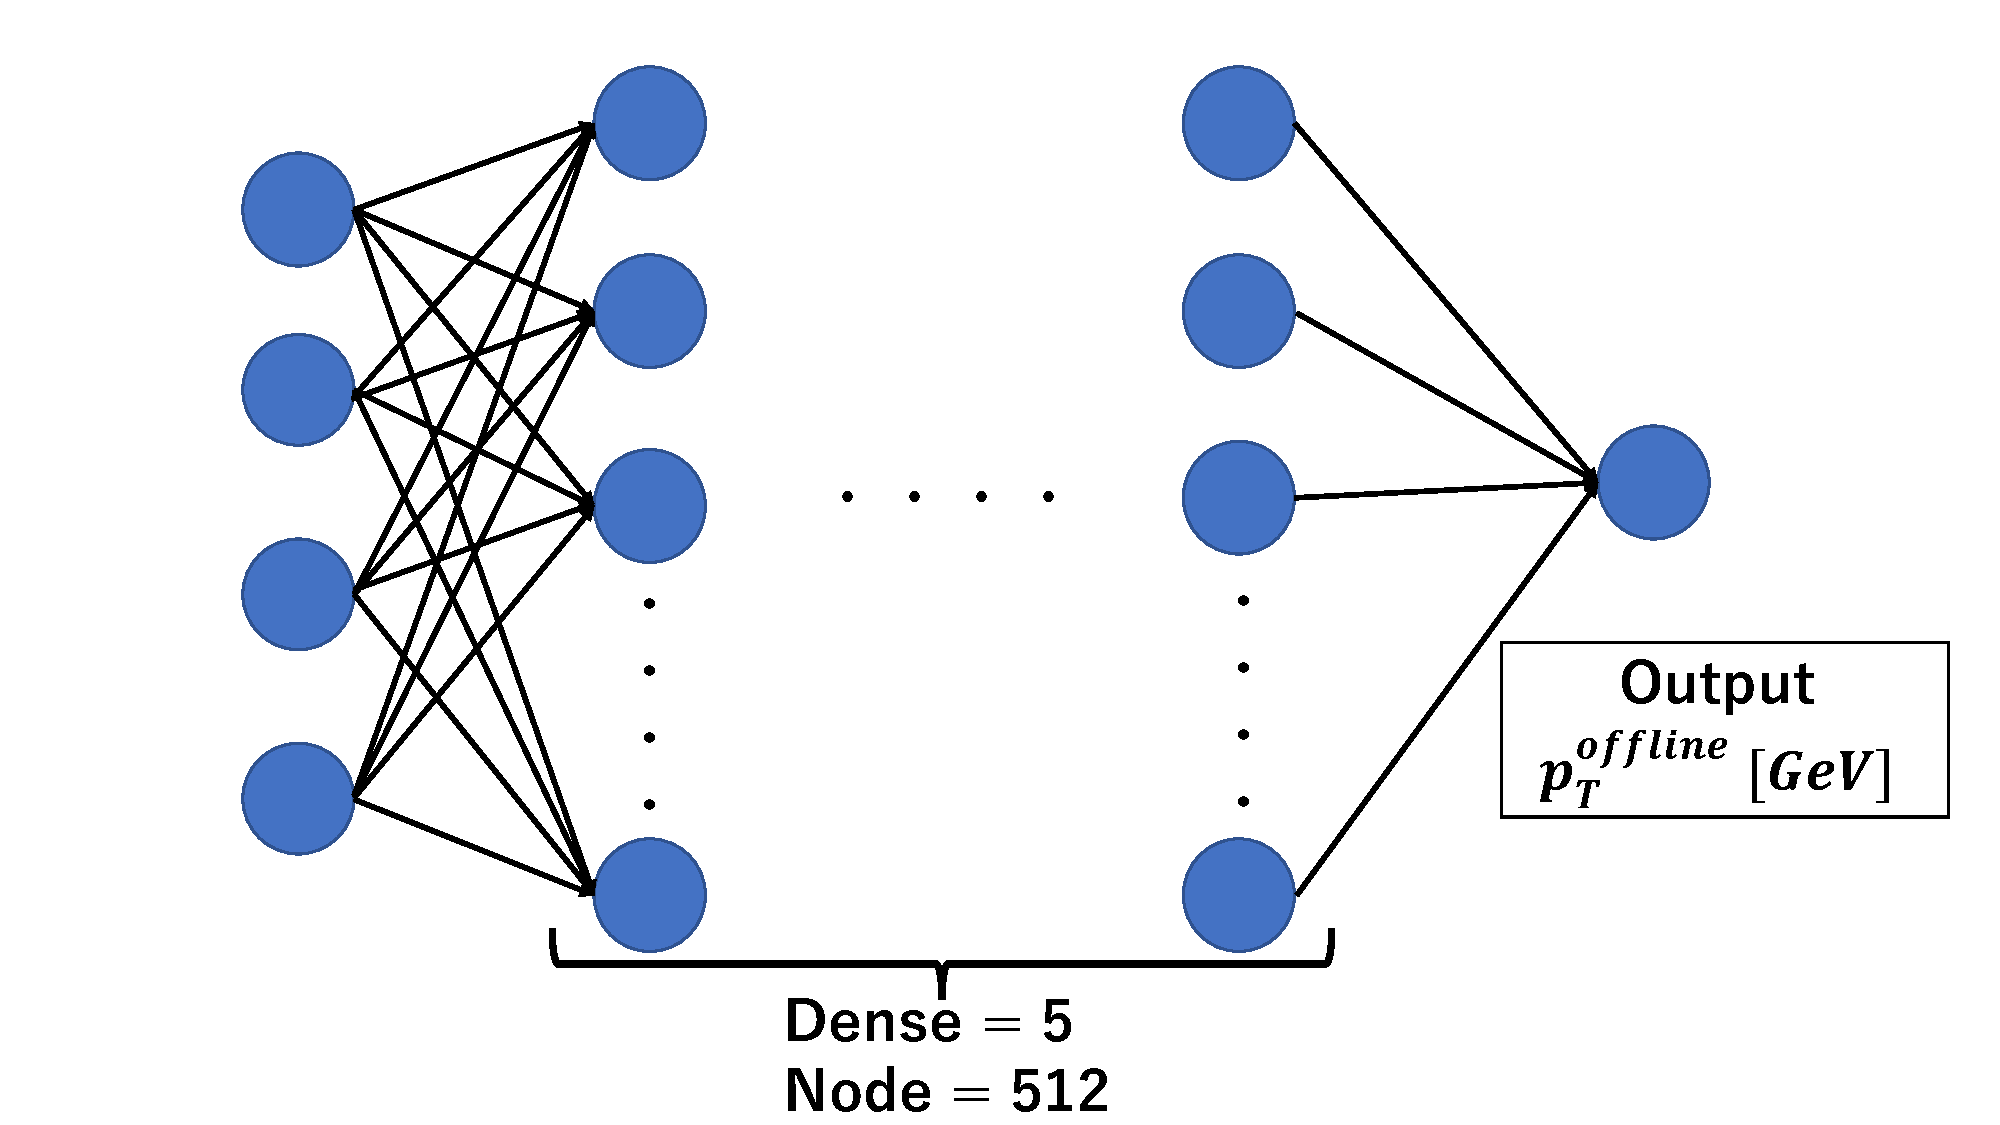
\includegraphics[clip, width=12cm]{fig/4/MLP.pdf}
  \caption{機械学習モデルの概要図。}
  \label{fig:MLP_overview}
\end{figure}


\subsubsection{トレーニング}



\begin{figure}[tb]
  \centering
  \rule{8cm}{6cm}
  %\includegraphics[clip, width=14cm]{}
  \caption{深層学習モデルのトレーニングに用いたミューオンサンプルの $p_T$ 分布。}
  \label{fig:mu_pt_forMC}
\end{figure}

\begin{figure}[tb]
  \centering
  \rule{8cm}{6cm}
  %\includegraphics[clip, width=14cm]{}
  \caption{深層学習モデルのトレーニングに用いたミューオンサンプルの $p_T$ 分布。}
  \label{fig:mu_pt_forData}
\end{figure}

トレーニングの際に設定した



\subsubsection{機械学習モデルの性能評価}



\begin{figure}[tb]
  \centering
  \rule{8cm}{6cm}
  %\includegraphics[clip, width=14cm]{}
  \caption{残差分布(MC)}
  \label{fig:fit_def}
\end{figure}

\begin{figure}[tb]
  \centering
  \rule{8cm}{6cm}
  %\includegraphics[clip, width=14cm]{}
  \caption{trueに対するpredの分布(MC)}
  \label{fig:fit_def}
\end{figure}

\begin{figure}[tb]
  \centering
  \rule{8cm}{6cm}
  %\includegraphics[clip, width=14cm]{}
  \caption{true-prepのpt分布(MC)}
  \label{fig:fit_def}
\end{figure}

\begin{figure}[tb]
  \centering
  \rule{8cm}{6cm}
  %\includegraphics[clip, width=14cm]{}
  \caption{残差分布(Data)}
  \label{fig:fit_def}
\end{figure}

\begin{figure}[tb]
  \centering
  \rule{8cm}{6cm}
  %\includegraphics[clip, width=14cm]{}
  \caption{trueに対するpredの分布(Data)}
  \label{fig:fit_def}
\end{figure}

\begin{figure}[tb]
  \centering
  \rule{8cm}{6cm}
  %\includegraphics[clip, width=14cm]{}
  \caption{true-prepのpt分布(Data)}
  \label{fig:fit_def}
\end{figure}


\subsection{出力データから CW の作成}
\subsubsection{出力データ}
\subsubsection{fitting}


4bit


・Efficiencyに対するfitting <fittingの定義のプロット><threshould><Resolution><プラトー>\\
\begin{figure}[tb]
  \centering
  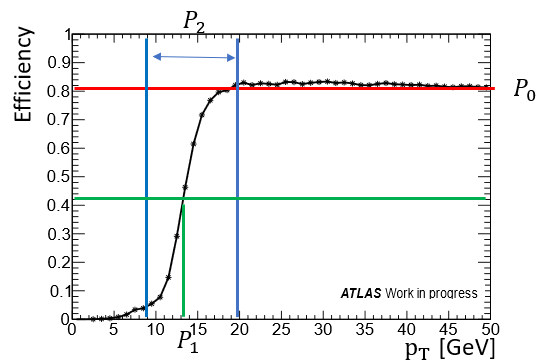
\includegraphics[clip, width=14cm]{fig/4/fitting_def.png}
  \caption{fittingの定義}
  \label{fig:fit_def}
\end{figure}

\begin{figure}[tb]
  \centering
  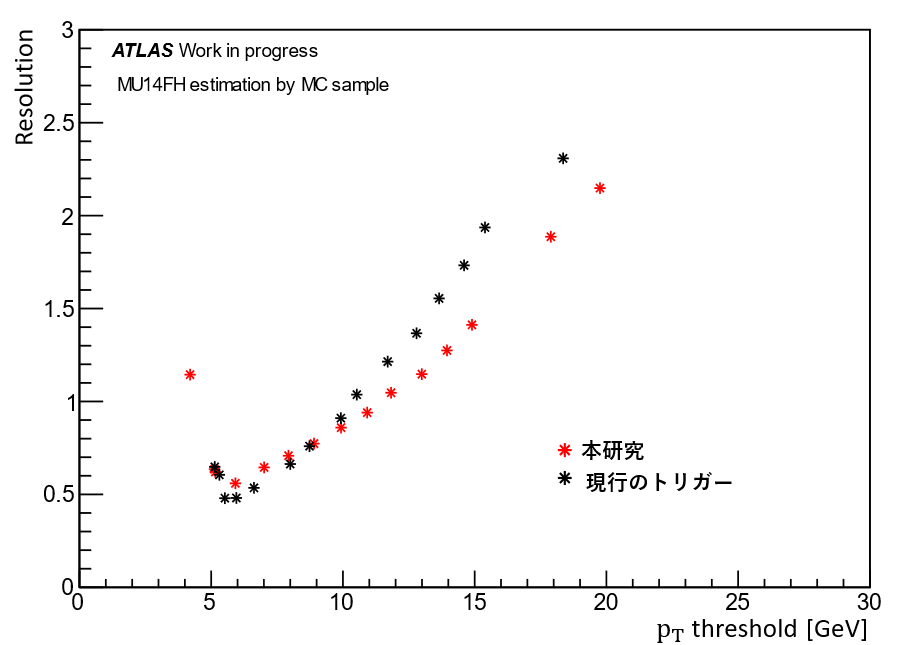
\includegraphics[clip, width=14cm]{fig/4/resolution_v07_v05.png}
  \caption{Resolution}
  \label{fig:Resolution}
\end{figure}

\subsubsection{出力データをPt閾値に変換}

